%!TEX root = ../dissertation.tex

\chapter{What is conceptual complexity?}
\label{chapter:complexity}

The studies in Chapter 2 provide robust evidence for a regularity between word length and a dimension of word meaning, complexity. In these studies, we operationalized the notion of complexity by manipulating the visual complexity of objects in terms of number of component parts. We found that the number of parts  positively correlated with participants' study time in a memory task, providing additional evidence that the stimulus complexity was psychologically relevant. Furthermore, we found that the notion of conceptual complexity extended beyond the visual domain to abstract word meanings in natural language. This finding points to a theory of conceptual complexity that is more general than simply the number of visual parts associated with an object.  Notably, however, this work leaves open the important question of what exactly this theory is---what makes one meaning more conceptually complex than another? Here we try to more directly address this question. 

To formalize the notion of complexity, we adopt an information theoretic approach \cite{shannon1948}. The central idea of Information Theory is that, within a communication channel, each meaning $m$ is communicated with probability $p$, such that the amount information conveyed by each occurrence of $m$ is $-log(p)$. Critically, if it is assumed that the overall length of the code in the communication channel is minimized, then meanings should be assigned to codes in a particular way: Less probable meanings should be assigned to longer codes. By making these assumptions, we establish a fundamental link between the amount of information in a code, its probability of occurrence and its length. In our work here, we appeal to this framework to derive a metric of complexity: More complex codes are longer, less probable, and contain more information.\footnote{This relationship is reflected in the idea of minimum description length proposed by Kolmogorov and others: In a maximally compressed code, more complex codes are longer.} 

Information Theory thus provides a  starting point for evaluating the complexity of a concept by providing a quantitative measure. But, an important property of this theory is that the metric of complexity depends on the representational framework. In other words, what counts as ``one unit" of code in the  channel depends on the representational system that is assumed. This representational agnosticism implies that a meaning that is relatively more complex in one representational framework may relatively less complex in another, or that  complexity in one representational framework may be entirely unrelated to conceptual complexity.

In the case of concepts, it is not a priori obvious what representational framework is most useful in describing their psychological status; what the ``communication channel" of concepts is. The most intuitive is perhaps the Classical View of concepts \cite{laurence1999concepts}, where the units of  representation are primitives and a language for combining them. To illustrate, consider the geon stimuli from Chapter 2:  If we assume that a ``unit" is equivalent to a geon,  then an object composed of a sphere and cone has a conceptual complexity of two, and an object composed of only a sphere, has a conceptual complexity of one. This is the representational framework that is most similar to the approach in Chapter 2. 

Importantly, however, the literature on concepts and categories has explored a range of alternatives to the Classical View \cite{laurence1999concepts}, which we consider in this chapter. In particular,  we consider how the following two views may be related to conceptual complexity:
\begin{quote}
	(1) {\it Classical View}: Concepts are represented as a structured set of primitives.\\
	(2) {\it Statistical View}: Concepts are represented as a set of individual exemplars (Exemplar Theory), or as summary descriptions of exemplars (Prototype Theory).
\end{quote}
We consider each of these views in the broadest form, abstracting away from the many variants within each theory. We then apply Information Theory to each view of concepts and ask what would make one concept more complex than another, assuming the representational framework of that theory. Briefly, for the Classical View, a more complex concept is one with a longer description length. For the Statistical View, a more complex concept is one with more stored exemplars (Exemplar Theory), or with more uncertainty (Prototype Theory). We return to these predictions in more detail below.

We see our goal as not  to distinguish between these  views , nor even that they are incompatible with each other \cite<e.g.,>{murphy2015there,briscoe2011conceptual}. Rather, we consider each of these views as paradigms, in a Kuhnian sense, and ask whether these frameworks can inform our understanding of conceptual complexity when considered in the context of Information Theory. Our approach will be to observe variability in the complexity of meanings as defined within a particular theory of concepts, and ask whether this variability is related to the length of the word that meaning is mapped to. Evidence that a manipulation of conceptual complexity is related to word length would shed light on the underlying construct of conceptual complexity.  

In what follows, we review previous work related to each broad view of concepts---Classical and Statistical---followed by  a series of empirical studies testing  predictions of each view. In total, we conduct seven studies exploring various predictions these theories (see Table~\ref{tab:complexity_pred_summary_table} for summary of our studies). We conclude with a brief summary of our results. 


\bgroup
\def\arraystretch{1.5}% 

\begin{table}[t]
%\footnotesize
\centering
\begin{tabular}{l l l l l }
 \toprule
 \textbf{View} &  \textbf{\begin{tabular}[c]{@{}l@{}}Relevant\\Dimension\end{tabular}} & \textbf{Prediction}& \textbf{\begin{tabular}[c]{@{}l@{}}Relevant\\Studies\end{tabular}} \\
 \toprule
Classical  & \# of primitives & \multicolumn{1}{p{5cm}}{Concepts with longer definitions (and thus more primitives) will be more complex.} & Studies 1-4 \\
Statistical: Exemplar   &  \# of exemplars & \multicolumn{1}{p{5cm}}{Concepts with more  exemplars will be more complex.} & Studies 5-6  \\
Statistical: Exemplar  & Variability of exemplars &\multicolumn{1}{p{5cm}}{Concepts with more variable exemplars will be more complex.} & Study 7 \\
Statistical: Prototype  & \# of exemplars & \multicolumn{1}{p{5cm}}{Concepts with fewer exemplars will have more uncertainty, and thus be more complex.} & Studies 5-6     \\
Statistical: Prototype  & Variability of exemplars &\multicolumn{1}{p{5cm}}{ Concepts with more variable exemplars will have more uncertainty, and thus be more complex.} & Study 7 \\

 \bottomrule
\end{tabular}
\caption{Summary of studies.}
\label{tab:complexity_pred_summary_table}
\end{table}
\egroup

\section{Classical View}
A concept in the Classical View is defined by a rule, or definition, composed of a structured set of conceptual primitives. These definitions are typically considered deterministic of category membership, but more recent work has considered this theory in a probabilistic framework \cite{goodman2008rational}.

This theory has been productively instantiated with Boolean concepts and first-order logic \cite{shepard1961learning,feldman2000minimization,goodman2008rational}.  In this  framework, there are a set of primitives concepts, or predicates, that are represented by binary features, and a syntax for combining them given by first order logic.  For example, consider the concept if \textsc{mother}: If \textsc{female} and \textsc{has\_child} were primitives in the representational language, then  \textsc{mother} would denote the set of people where both primitives were true. 

The information theoretic measure of complexity falls straight-forwardly out of this formulation: Concepts defined by more primitives are more complex \cite{shepard1961learning,feldman2000minimization,goodman2008rational}. In the  above example, then, the complexity of the concept  \textsc{mother} would be two. Consistent with this proposal, there is evidence to suggest that the difficulty of acquiring a concept scales with its conceptual complexity: Concepts that are more difficult to learn tend to have longer definitions\cite{shepard1961learning,feldman2000minimization}.

An important issue for this theory of concepts is identifying a general set of conceptual primitives. Although this task might rank among the deepest challenges for cognitive science, some work has attempted this task. A body of research has sought to understand the innate conceptual primitives in young children (``core knowledge''; Kinzler \& Spelke, 2007). \nocite{kinzler2007core} The proposed set of concepts in this work, however, is restricted to those present only  in early development (e.g., ``agent"), and is therefore not suitable for the broad scope of our current project.  Wierzbicka and colleagues (1996) have also  sought  to identify conceptual primitives, but with a more general focus.  \nocite{wierzbicka1996semantics} This work compares lexical systems across languages  to identify common primitives. The hypothesis is that there exists universal and innate semantic primitives which are the building blocks of meaning in human language. Under this view, all meanings can be derived from a set of numerable semantic primitives and a syntax for combining them.

A related issue is whether the set of primitive concepts  changes over time: Might the conceptual complexity of a concept reduce with experience? That is, might a concept that is initially complex reduce in  complexity, such that it itself becomes an atomic unit in other concepts? This possibility is intriguing, but it remains an open question what sort of experience might lead to a reduction in complexity. One possibility is that the very act of labeling a concept reduces the complexity of a concept\cite{bruner1956austin}. This proposal is consistent with a large body of literature suggesting advantages in concept learning for labeled as opposed to unlabeled categories \cite<e.g.>{balaban1997,lupyan2007,sloutsky2001}. 

However, there is reason to think that other aspects of experience might affect the conceptual complexity of concepts since the length of words can change over time. For example, the word ``telephone" has become more typically ``phone" in standard usage. This type of  diachronic reduction in word length may be due to factors  unrelated to conceptual complexity (e.g.\ frequency of usage), but it might also reflect a decrease in conceptual complexity due to experience, beyond simply tokening the concept. Our work here does not directly address the character of the underlying  primitives, nor whether they are universal or innate or change over time. Rather, it assumes only that such units exist for a speaker and that lexical meanings can vary in the number of their compositional primitives. 

Motivated by the Classical View of concepts, Studies 1-4  explore whether the definition length of a concept  is related to the length of the label denoting that concept. In these studies, we assume that words denote conceptual units, such that concepts associated with longer linguistic definitions are  more complex. We find some evidence in support of this hypothesis.


%``length of the shortest Boolean formula logically equivalent to the concept"

%- Evidence consistent with that: Feldman (Boolean) - learning difficult

%- Issue: where do primitives come from? Might be related to experience. If we new what they were


%\cite{laurence1999concepts,anaki2009familiarity,feldman2016simplicity,goodman2008rational,haskell2011linguistic,lupyan2008conceptual,feldman2000minimization}

%Psychological metrics of complexity - trasnfer vs. recognition. 

%If, however, we assume a different representational framework, we might code this same object with a single conceptual primitive, ``ice cream cone."

\subsubsection{Experiment 1: Descriptions of objects}
In Chapter 2, we presented participants with novel, real objects and measured their complexity through explicit judgements (Exp.\ 4; pg.\ \pageref{ch2-4}) and study time (Exp.\ 8b; pg.\ \pageref{ch2-8b}). Both of these measures showed variability, suggesting that these objects differed in their complexity. 
In Experiment 1, we consider this result in the context of the Classical View of concepts. The Classical View suggests that these objects differ in complexity because they are composed of different number of conceptual primitives, with more complex objects containing more primitives that simpler objects. We reasoned that, if true, these primitives should be reflected in participants linguistic descriptions of the objects. In particular, we predicted that objects rated as more complex and studied longer in Exp.\ 4 and 8b should also be described with longer descriptions. We test this prediction here by asking participants to produce written linguistic description of the objects.


\subsection{Methods}
\subsubsection{Participants} 
In this and all subsequent experiments, participants were recruited on Amazon Mechanical Turk and received US \$0.15-0.50 for their participation, depending on the length of the task. 60 participants completed this first experiment.
\subsubsection{Stimuli} 
We used the same set of 60 novel real objects as in Chapter 2 (Fig. \ref{fig:realobjs}; pg.\ \pageref{fig:realobjs}).

\subsubsection{Procedure}
On each trial, we presented a single object and following instructions:  ``Look at the object below. Imagine you just received this object as a gift. Describe what the object looks like to a friend." Participants then entered their description in a text box below the object.

Each participant described 10 objects in total. Five objects were from the top quantile (high complexity) and 5 objects were from the bottom quantile (low complexity). Order of objects was randomized across trials.

\subsection{Results and Discussion}


\begin{table}[t!]
\centering

\begin{tabular}{ll}
\toprule
\multirow{6}{*}{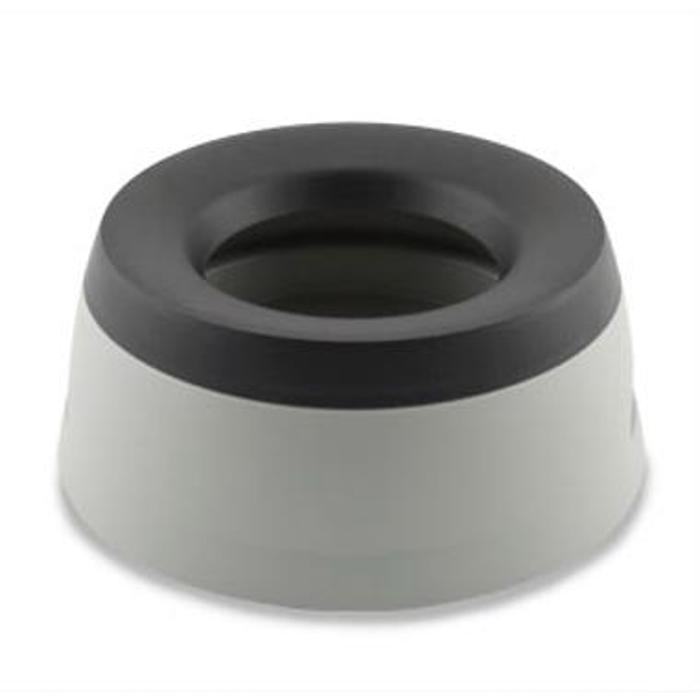
\includegraphics[width=2cm]{figs/obj_29_p2.jpg}} & \textbf{Low-complexity object}                \\
\toprule
                   & ``cup holder"                                   \\
                   & ``it is a bowl with a black portion on top"      \\
                   & ``football kicker's stand"                      \\
                   & ``a hole type thing"                              \\
                   & ``it looks like an ash tray, but a bit shallow" \\
                   & ``looks like a dog bowl" \\
 \bottomrule
~ & ~ \\
  \toprule
\multirow{6}{*}{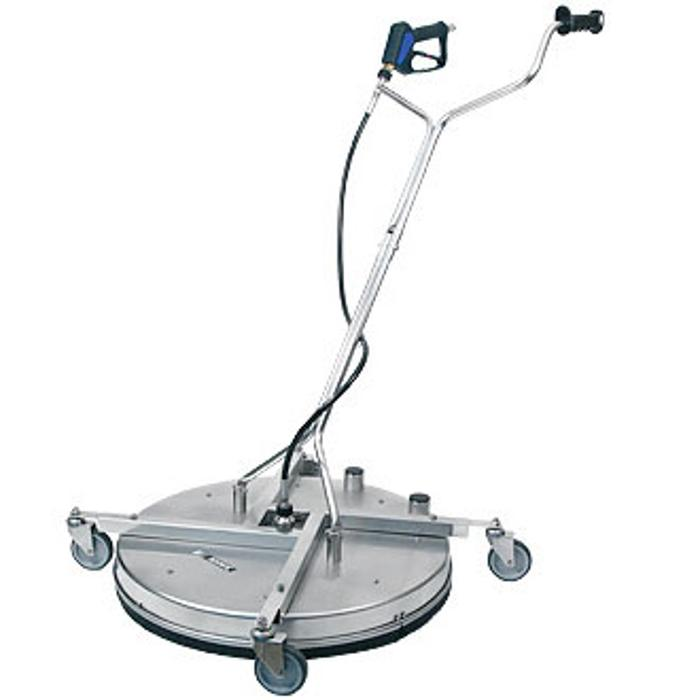
\includegraphics[width=1.8cm]{figs/obj_27_p2.jpg}} & \textbf{High-complexity object}               \\
\toprule
                   & ``a robotic carpet shampooer"                                   \\
                   & \multicolumn{1}{p{12cm}}{ ``it's a flat silver disk on rollers with what appear to be tall handlebars standing away from it at an angle"}                     \\
                   & ``a pressurized floor buffer on wheels"                                   \\
                   & ``it looks like a high tech metal detector on wheel."                                   \\
                   & ``it kinda looks like a portable lamp"                                \\  
                   & ``it is a machine with a circular stand and wheels, it has a metal handle"\\
   \bottomrule
\end{tabular}
\caption{Sample descriptions of a low- (top) and high- (bottom)  complexity objects.  Overall, descriptions were longer for high-complexity objects.}
\label{tab:sample_obj_descriptions}
\end{table}


Example descriptions for a sample low and high complexity object are presented in Table~\ref{tab:sample_obj_descriptions}. We considered two measures of length:  log number of words and log number of characters. Across objects, the mean length of description was  $8.82$ words ($SD = 1.14$) and $36.31$ characters ($SD = 4.69$).

 \begin{figure}
 \begin{center}
  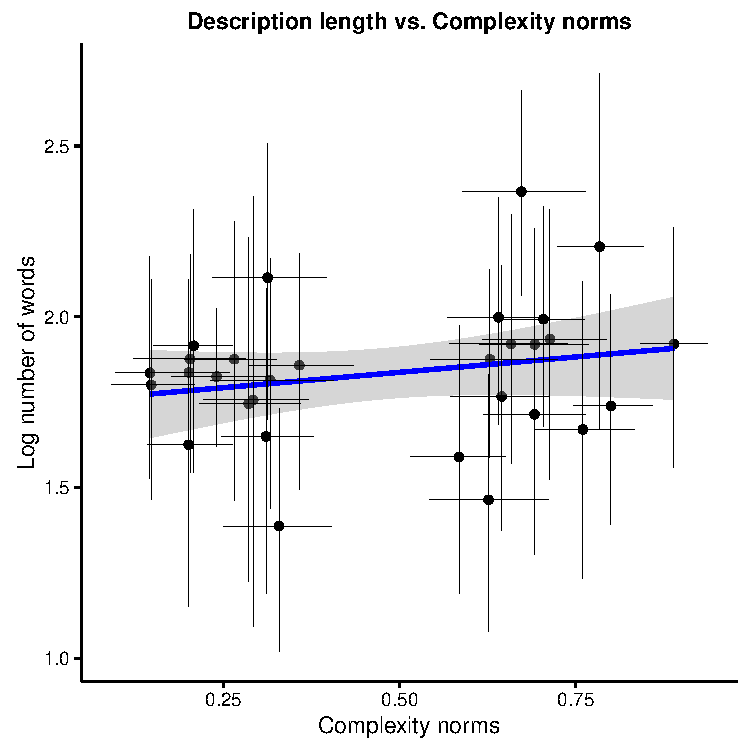
\includegraphics[width=4in]{figs/desc_length_word.pdf}
  \caption{\label{fig:desc_length} Relationship between description length and complexity norms. Error bars show  95\% confidence intervals.}
 \end{center}
\end{figure}


The key question was whether the description length was related to the psychological correlates of complexity measured in Chapter 2, explicit ratings and study times.
To test this question we fit a  linear mixed-effect model predicting log number of words with complexity norms as a fixed effect, and a second model predicting log number of words with study times as a fixed effect. As evident from Table~\ref{tab:sample_obj_descriptions}, participants varied considerably in the  syntactic construction of their descriptions as well as overall  length, making it important to control for this variability using a  mixed-effect model. The random effect structure included by-participant intercepts and by-trial slopes. There was a reliable relationship between log number of words and  complexity norms ($\beta=.2$, $t =2.8$; Fig~\ref{fig:desc_length}), and between log number of words and log study time ($\beta=.59$, $t =3.07$). The same pattern held for log number of characters. 

In the context of the Classical View of concepts, this result suggests a connection between conceptual complexity and number of primitives: More conceptually complex objects have longer descriptions, and thus more primitives. 

\section{Experiment 2a: Definitions of words}
Experiment 1 suggested objects that appear visually more complex are described with longer descriptions. The studies in Chapter 2, however, suggest that the construct of conceptual complexity extends beyond visual complexity to abstract word meanings. This predicts that the length of a dictionary definition of a word should be correlated with the conceptual complexity of its meaning. In light of the complexity bias observed in Chapter 2, we also predict that words with more complex definitions should be longer and have definitions that are rated as more complex. In Experiment 2 we tested these predictions by presenting participants with the definition of low frequency English words  and asking them to rate the conceptual complexity of the definition.

We selected low frequency words for several reasons. First, because participants were unlikely to know the word associated with the definition, knowledge of a word's length was unlikely to affect the complexity judgement. Second, because the words were uniformly low frequency, this reduced the possibility that differences in word length were due to frequency, rather than conceptual complexity. Finally, because participants were unlikely to know the words, we could conduct a follow-up experiment (2b) probing judgements about the length of a meaning's word, without knowledge of the English word interfering with this judgement.

\subsection{Methods}

\subsubsection{Participants} 
200 participants completed the task.

\subsubsection{Stimuli} 
We selected 100 dictionary definitions of low-frequency words (see Table~\ref{tab:sample_word_defs} for examples). 

\begin{table}[t!]
\centering

\begin{tabular}{ll}
\toprule
\textbf{Word} & \textbf{Definition}                \\
\toprule
   bissextile & ``a leap year"\\
   mussitation  &  \multicolumn{1}{p{12cm}}{ ``movement of the lips as if in speech but without accompanying sound"}    \\
   omphaloskepsis  &  \multicolumn{1}{p{12cm}}{ ``contemplation of one's navel as an aid to meditation"}                  \\
   parvis    &  \multicolumn{1}{p{12cm}}{ ``a court or enclosed space before a building"}                               \\
   sniddle      &  \multicolumn{1}{p{12cm}}{ ``long coarse grass"}     \\
   zarf     & \multicolumn{1}{p{12cm}}{ ``a holder, usually of ornamental metal, for a coffeecup without a handle"}                                 \\

 \bottomrule
\end{tabular}
\caption{Sample definitions of real English words used in Experiment 2.}
\label{tab:sample_word_defs}
\end{table}


\subsubsection{Procedure}
The task was identical to Experiment 9 in Chapter 2 (pg.\ \pageref{ch2-9}), except that participants were presented with definitions rather than words. Participants were first presented with instructions describing the norming task:
\begin{quote}
In this experiment, you will be shown the definition of a word and asked to decide how complex the meaning is. A word's meaning is simple if it is easy to understand and has few parts. An example of a simple meaning is ``brick.'' A word's meaning is complex if it is difficult to understand and has many parts. An example of a more complex meaning is ``engine.''
\end{quote}
For each definition, we then asked ``How complex is this definition?,'' and participants indicated their response on a 7-pt Likert scale anchored at ``simple'' and ``complex.'' The first two words were always ``ball'' and ``motherboard'' to anchor participants on the scale. Each participant rated a sample of 10 definitions. 

\subsection{Results and Discussion}
The central prediction is that definitions with more primitives in the definition, operationalized as the length of the definition, should be rated as conceptually more complex. To test this prediction, we fit a linear mixed-effect model predicting complexity ratings with log number of words in the definition as a fixed effect. The random effect structure included by-participant intercepts and by-trial slopes. As predicted, there was a strong relationship between complexity ratings and log number of words ($\beta=1.50$, $t =27.94$). The same pattern held for log number of characters.

A secondary prediction is that there should be a relationship between the length of the definition and the length of the word: If languages encode the conceptual complexity of a word's meaning in the length of the word, longer words should be associated with longer definitions. This prediction was not supported ($r=.05$, $p =.59$). Finally, we should also expect that  longer words should be associated with definitions rated as more complex. We fit the same mixed-effect model as above to test this prediction, except with log number of characters in the word as a fixed effect. There was a significant relationship between word length and rating judgements ($\beta=.52$, $t =2.86$), suggesting more complex definitions area associated with longer words. However, in a model with both word length and definition length as fixed effects, word length was no longer a reliable predictor of complexity ratings ($\beta=.18$, $t =1.19$).

In sum, we find a strong relationship between definition length and conceptual ratings, as predicted by Classical View of concepts: Longer definitions, with more primitives, are rated as more complex. We do not, however, find the predicted relationship between the conceptual complexity of the definition and word length, as would be predicted by the studies in Chapter 1.  One possible explanation for this null finding is that participants' complexity ratings were driven by the linguistic complexity of the definition, rather than its conceptual complexity. In other words, participants may have  rated longer definitions as more complex {\it because} they were longer, not because they were more conceptually complex. The current design does not allow us to distinguish these two possibilities.

\section{Experiment 2b: Definition mapping}
If definition length is related to conceptual complexity and participants have a complexity bias, we predict that participants should be biased to map more complex definitions on to longer words. In Experiment 2b, we test this prediction in an experiment analogous to the word mapping experiments in Chapter 2. Participants were presented with a meaning---a definition---and asked to guess the translation of the meaning in an alien language from two possible alternatives, one long and one short. 

\subsection{Methods}
\subsubsection{Participants} 
200 participants completed the experiment.
\subsubsection{Stimuli} 
We used the normed definitions from Experiment 2a. The short novel words contained one syllable, and the long novel words contained three syllables. There were 10 short and 10 long novel words presented in random order. 

\subsubsection{Procedure}
Participants were first presented with the following instructions:
\begin{quote}
In this experiment, you will see the definition of a word. Your job is to guess what the translation of that word is in an alien language. You will make your guess by betting on two possible words in the alien language. Imagine you have a \$100 dollars. To place your bet, assign an amount to each of the words. Your bets must add to 100.
\end{quote}
Participants then viewed a definition and two possible alternative words, one short and one long. Participants selected a response by placing a numeric bet (0-100) under each word.  Each participant rated 10 definitions in total. 

\subsection{Results and Discussion}
Consistent with previous evidence, we found a complexity bias in participants mappings from definition to words: Participants tended to map definitions rated as more complex in Experiment 2a to longer words ($r = .39$,  $p< .0001$). However, there was also a strong correlation between participants bets to longer words and definition length, measured in terms of log number of characters ($r = .82$, $p< .0001$). In an additive linear model predicting bets to the long word with both complexity norms and definition length, definition length ($\beta=3.81$, $t =2.64$, $p<.01$) was a significant predictor of bets, but complexity norms were not ($\beta=1.02$, $t =1.38$, $p=.17$). 

While this result is consistent with a complexity bias, as well as the pattern of complexity predicted by the Classical View of concepts, it is difficult to make strong causal inferences from these data. The fact that definition length accounts for more variance in bets than complexity norms suggests that it may be linguistic complexity, rather than conceptual complexity that is driving this bias. This result may simply reflect participants bias to map long definitions to long words. While a positive finding, this result does not speak to the claim directly that it is {\it conceptual} complexity per se that is related to definition length and the bias in word length. In Study 3, we try to address this issue more directly. 

\section{Study 3: Feature norms}
Study 3 provides tests the Classical View of complexity by examining the conceptual primitives of a concept through feature norms. Feature norms are collected by presenting participants with the name of a concept (e.g., ``moose") and asking them to produce as many features of the concept as possible (e.g., ``has for legs", ``has antlers"). If we assume that the features participants generate correspond to conceptual primitives in the definition of that concept, then the Classical View of concepts predicts that concepts with more  features should be more conceptually complex. If true, we should also expect concepts associated with more features to have longer labels. We test this prediction using a set of previously-collected feature norms.

\subsection{Method}
We analyzed feature norms for a set of 541 nouns \cite{mcrae2005semantic}. For each noun concept, we examined the relationship between the length of the word and the number of unique features participants listed for that concept. A feature was excluded from this measure if it was listed by fewer than 5 of 30 participants or described a taxonomic associate of the concept (subordinate or superordinate). Taxonomic associates were excluded because they are conceptually different than features which describe parts and functions. Word length was measured in terms of log number of characters. We also included spoken frequency of the target noun as a covariate in our models, measured from the Subtlex-us database \cite{brysbaert2009moving}. 

\subsection{Results and Discussion}
We first analyzed the simple correlation between word length and the number of features and found no relationship ($r=-.03$, $p=.54$)  However, spoken frequency is a strong, independent correlate of word length \cite{zipf1936}, and so it is important to control for this variability in measuring the relationship between number of features and word length. We fit an additive linear model predicting word length with both log spoken frequency and number of features.  There was a  relationship between number of features and word length (Fig.\ \ref{fig:feature_plot}): Longer words tended to have more features. Model parameters are presented in Table~\ref{study3amodel}.\footnote{We also fit the same model with the measure of number of features that included taxonomic features. In this model, the relationship between length and number of features was marginal ($\beta=0.08$, $t =1.92$, $p=.06$).} 

  \begin{figure}
 \begin{center}
  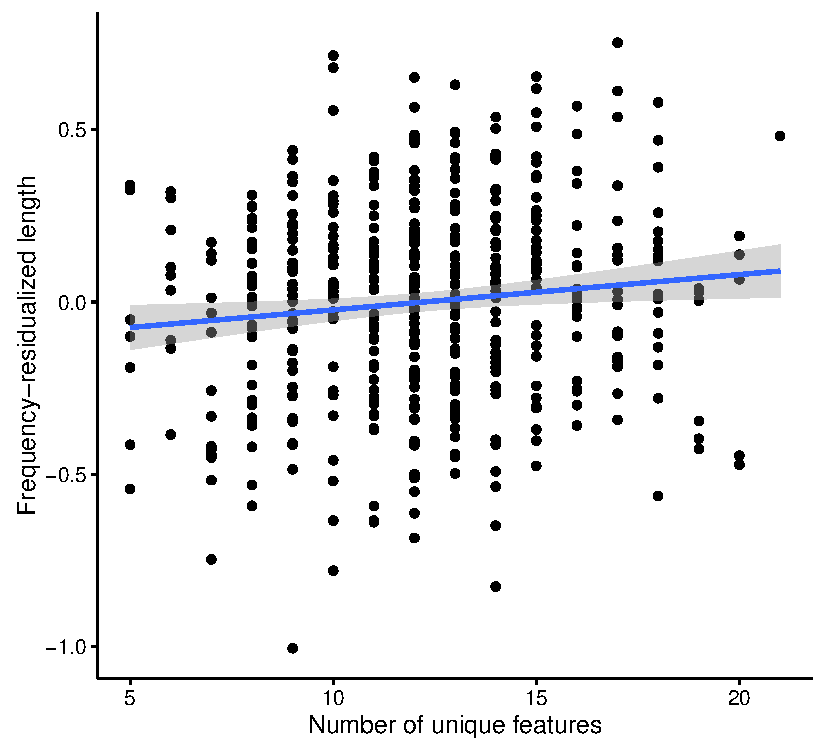
\includegraphics[width=4in]{figs/feature_plot.pdf}
  \caption{\label{fig:feature_plot} Study 3 results: Frequency-residualized word length (measured in log number of characters) as a function of the number of unique features associated with the concept a word denotes. }
 \end{center}
\end{figure}

% latex table generated in R 3.3.0 by xtable 1.8-2 package
% Mon Oct 10 13:57:56 2016
\begin{table}[t!]
\centering
\begin{tabular}{rrrrr}
  \hline
 & Estimate & SE & t-value & p-value \\ 
  \hline
(Intercept) & 2.2411 & 0.0638 & 35.13 & $<.001$ \\ 
  Num. features & 0.0112 & 0.0043 & 2.59 & $<.01$\\ 
  Log frequency & -0.2626 & 0.0214 & -12.29 & $<.001$  \\ 
   \hline
\end{tabular}
\caption{Model parameters for linear regression predicting word length in terms of number of features, controlling for word frequency.}
\label{study3amodel}
\end{table}

This finding is consistent with the Classical View, and suggests that conceptual complexity may be associated with the number of ``primitive" features associated with a concept.

\section{Study 4: Concept associates}
One limitation of Study 3 is the relatively small set of words used in the dataset. In Study 4, we aimed to replicate Study 3 with a larger dataset. We analyzed data from a word-association dataset in which participants were presented with a word asked to generate three ``related" words. This task differs notably from the feature norms in that participants were allowed to generate any word related to the target, not simply ``features" that describe conceptual parts. While this is a potential limitation of the current approach, we note that the distinction between features and associates is fuzzy. We find  the same pattern as in Study 3: Longer words tend to have more associates. 

The larger set of cue words in this dataset allowed us to also examine the relationship between the explicit complexity norms collected in  Experiment 9 in Chapter 2 (pg.\ \pageref{ch2-9}) and the number of associates. We reasoned that if the number of associates was related to conceptual complexity, as predicted by the Classical View,  these two variables should be positively correlated. This prediction was also supported.

\subsection{Method}
We analyzed an existing dataset containing word associations for  10,050 English words, collected from 73,256 participants \cite{de2013better}. The words include all grammatical classes. In the task, participants were presented with a cue and  asked to type ``the first  three words that came to mind." Each participant completed 15-19 trials. As in Study 3, we used a measure of spoken word frequency from the Subtlex-us database \cite{brysbaert2009moving}. 

\subsection{Results and Discussion}
We first tested for a relationship between log word length and number of unique associates: Word length was positively correlated with number of associates ($r = .11$, $p< .5$; see Table~\ref{study4corr} for all correlations).  Next, in order to control for the effect of word frequency on length, we fit an additive linear model predicting word length with number of associates and word frequency. Controlling for frequency, the relationship between number of associates and word length remained reliable ($\beta=0.004$, $t =27.34$, $p<.0001$; Fig.\ \ref{fig:associate_plot}).

Finally, we examined the relationship between the conceptual complexity norms from  Experiment 9 in Chapter 2  and number of associates. There were 431 words that overlapped between the two datasets. As predicted, there was a strong correlation between the conceptual complexity norms and number of associates: Words rated as more conceptually complex tended to have more associates ($r = .23$, $p< .0001$).


% latex table generated in R 3.3.0 by xtable 1.8-2 package
% Mon Oct 10 16:07:48 2016
\begin{table}[t!]
\centering
\begin{tabular}{llll}
  \hline
 & Log length (char.)  & Complexity norms &   Num. associates  \\ 
  \hline
Log length (char.) &  &  &  \\ 
Complexity norms  &  0.61**** &  &  \\ 
Num. associates &  0.11*    &  0.23**** &  \\ 
Log frequency& -0.54**** & -0.33**** &  0.18**** \\ 
   \hline
\end{tabular}
\caption{Pairwise correlations in Study 4. $p<.05$ = *; $p<.0001$ = ****}
\label{study4corr}
\end{table}

  \begin{figure}
 \begin{center}
  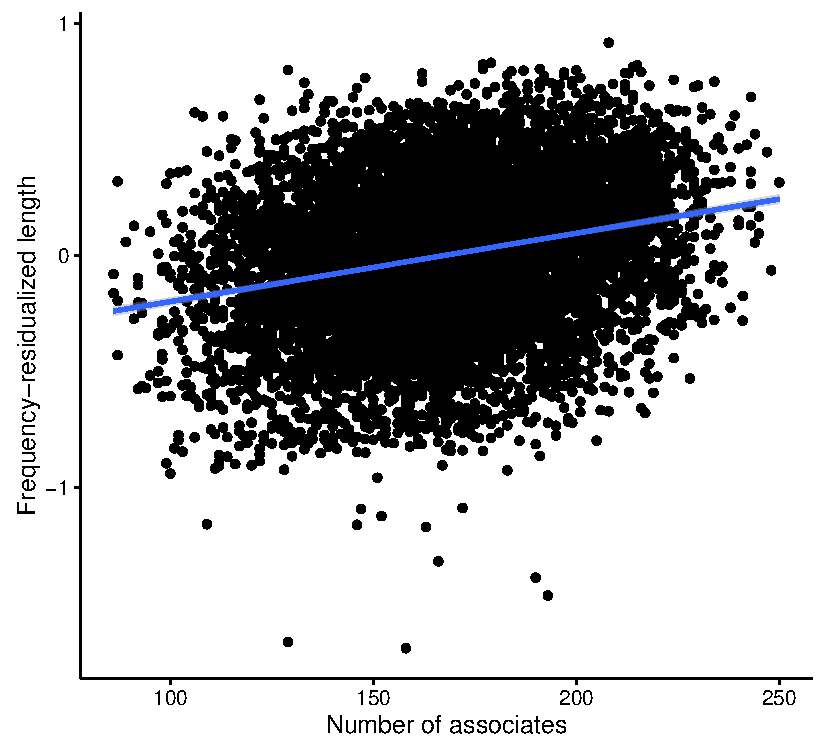
\includegraphics[width=4in]{figs/associate_plot.pdf}
  \caption{\label{fig:associate_plot} Study 4 results: Frequency-residualized word length (measured in log number of characters) as a function of the number of unique associates for a cue word. Each point corresponds to a word. For visualization, outliers three or more deviations above or below the mean were removed.}
 \end{center}
\end{figure} 

%Limit of this test of the classical approach -- assumes features are linguistically based; may not be true.

\section{Statistical View}
INTRO THE THEORIES
Exemplar + frequency
prototype + frequency
exemplar + variability
protype + variabiliyy

Exemplar Theory provides a second paradigm for considering the relative complexity of concepts. In this framework, a concept is represented as the set of individual exemplars observed of that category, with no additional compression of the concept in long term memory \cite<e.g.,>{medin1978context}. To operationalize complexity in this framework, we can again apply the description length criteria of Information Theory. If the primitives of representation are individual exemplars, then a more complex concept is one with more stored exemplars. W

How does frequency relate to concept learning. 
Evaluate: ease of learning model vs. transfer
Salthouse (1977): more exemplars increases recognition reaction time for letters, but NOT dot patterns (a concept) [same holds for accuracy)
Difference goes away with only a little bit of exposure
Argue there is an effect of number of exemplars only early in learning 

- More exemplars more transfer; worse memory for individual exemplars (see Omohunder, 1981; King and Newman, 1982)
- Familiarity speeds visual search paradigms (Wang, Cavaneough, Green 1994 ) 
- named famileiar matters more (Lupyan, 2008)


Salthouse (1977): more exemplars increases recognition reaction time for letters, but NOT dot patterns (a concept) [same holds for accuracy)
Difference goes away with only a little bit of exposure
Argue there is an effect of number of exmplars only early in learning 

\section{Experiment 5a: Simultaneous frequency}
We now turn to predictions about conceptual complexity from other theories of concepts: Exemplar and prototype theories. Both of these theories predict that aspects of experience should influence the representation of a concept, and thus the conceptual complexity of the concept. In particular, each makes predictions about the influence of observing individual exemplars of a concept.  Importantly, however, these two theories make different predictions about the direction of this influence. Under the exemplar theory, a participant who observes more exemplars of a concept consequently would have a representation of the concept that contained more individual exemplars. This is the case of an expert: A person who is a bird expert, for example, would have many exemplars of birds as part of the concept bird. This might mean that this concept has overall higher fidelity, than for a non-bird expert. Thus, the exemplar theory predicts that concepts with more observed exemplars will be more complex.

In contrast, the prototype theory predicts that participants represent only summary statistics over exemplars. If true, this means that the more exemplars a participant observes the less uncertainty there will be about the underlying concept; the concept prototype. Thus, the prototype theory predicts that the more exemplars a participant observes from a given concept, the {\it less} conceptually complex that concept will be. This prediction also falls out of an information theoretic account: Objects that appear more frequently are less surprising, and thus less conceptually complex.

In Experiment 5, we explore the possibility that the number of exemplars a participant observes influences the conceptual complexity of the concept. We present participants with either a few or many exemplars of a concept, and then ask participants to map that concept to either a short or long label. Under either theory, if conceptual complexity is related to exemplar frequency, we should expect the number of exemplars observed to influence how a concept is mapped to words of varying length. Under the exemplar theory, we expect long words to map to concepts with many exemplars, and under the prototype theory, we expect long words to map to concepts with few exemplars.

\subsection{Methods}
\subsubsection{Participants} 
477 participants completed the experiment.
\subsubsection{Stimuli} 
The objects were composed of a single geon, similar to those used in Expts.\ 1-3 in Chapter 2. The linguistic stimuli were novel words composed of either 2 (e.g., ``tupa," ``gabu," ``fepo")  or 4  (e.g., ``tupabugorn," ``gaburatum," ``fepolopus")  syllables.

\subsubsection{Procedure}
We presented participants with 10 objects on a single screen with a cover story that the objects were from a character's box (see Fig.\ \ref{fig:seqfreq_display} for precise text). Participants were required to click on a question mark to reveal each object. There were always two types of objects, one appearing nine times and the other once. Order of presentation was randomized.

After this training phase, participants completed a forced choice mapping task, as in Studies 1 and 5 in Chapter 2 (pg.\ \pageref{ch2-1} and pg.\ \pageref{ch2-5}). We presented a short or long word and asked participants to make a judgment about whether the word referred to the low or high frequency object. Each participant completed a single mapping trial, and word length was manipulated between participants.

 \begin{figure}
 \begin{center}
  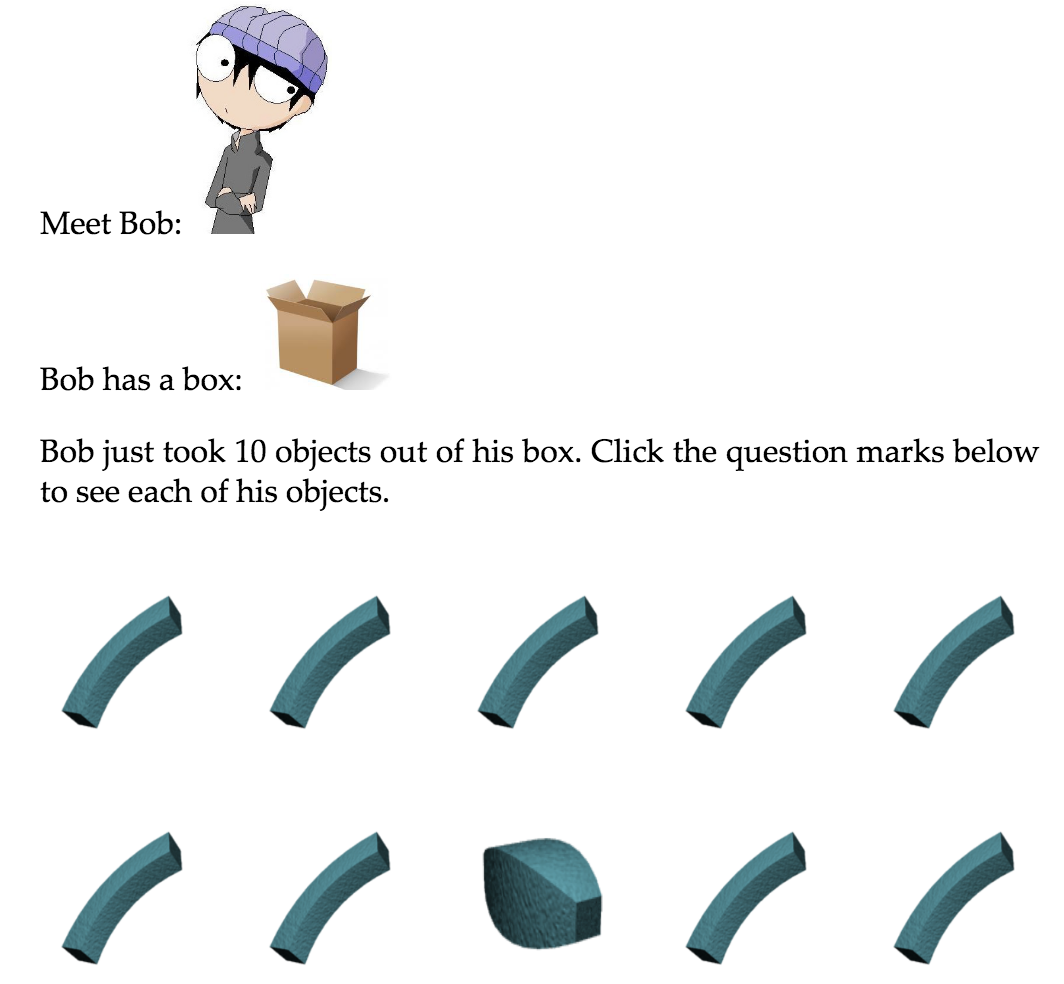
\includegraphics[width=3.5in]{figs/seqfreq_display.png}
  \caption{\label{fig:seqfreq_display} Sample display of the training phase in Experiment 5a.}
 \end{center}
\end{figure}


 \subsection{Results}
 Selections between the two conditions did not differ (${\chi}^2$$(1) = 0.02$, $p = .89$; Fig.\ \ref{fig:freq_plots}, left).
 
  \begin{figure}
 \begin{center}
  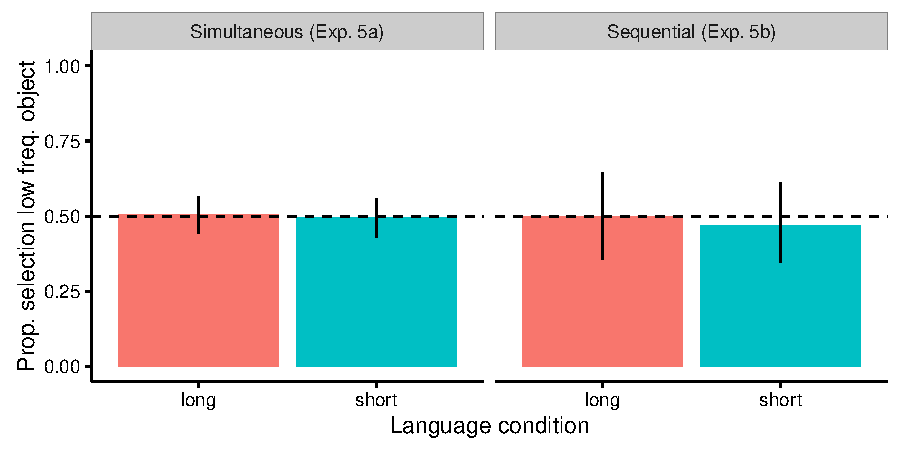
\includegraphics[width=6in]{figs/freq_plots.pdf}
  \caption{\label{fig:freq_plots} Proportion participants selecting the low frequency object as a function of language condition, in Exp.\ 5a (left) and Exp.\ 5b (right). Error bars are bootstrapped 95\% confidence intervals.}
 \end{center}
\end{figure}



\section{Experiment 5b: Sequential frequency}
Given the null finding in Experiment 5a, we next explore whether the timing of the presentation of exemplars affects complexity. Previous work has shown that participants may induce different concepts depending on whether or not exemplars are presented simultaneously, as in Exp.\ 5a,  or sequentially \cite<e.g.>{spencer2011}. In Experiment 5b, we present exemplars sequentially such that only one exemplar is visible at any given time. 

\subsection{Methods}
\subsubsection{Participants} 
97 participants completed the experiment.
\subsubsection{Stimuli} 

The objects were the set of novel, real objects used from Chapter 2, Expts.\ 4-6. 

\subsubsection{Procedure}
We manipulated object frequency by sequentially presenting objects. Participants saw 60 objects one at a time for 750 ms per object. One object was presented 10 times and a second object was presented 40 times. Ten additional objects were included as fillers, each appearing once. These were included to make the critical manipulation less obvious. Order of presentation was randomized. After this training phase, participants completed a single mapping trial as in Experiment 5a. Word length was manipulated between participants.

\subsection{Results and Discussion}
Selections between the two conditions did not differ (${\chi}^2$$(1) = 0.01$, $p = .92$; Fig.\ \ref{fig:freq_plots}, right). Across Expts.\ 5a and 5b, we find no evidence that the frequency of exemplars is related to the conceptual complexity of objects.

\section{Experiment 6: Facts}
In Experiment 6, we again test the hypothesis that the number of observed exemplars is related to conceptual complexity, as predicted by both the exemplar and prototype theories. However, in the present experiment, we explore the possibility that perhaps raw number of times an exemplar is observed is not the psychologically relevant dimension of frequency. We instead ask whether {\it conceptual} frequency, or markedness, is related to conceptual complexity by teaching participants facts about novel objects. We selected four categories of facts  that indicated the frequency of the object in the world, in a psychologically relevant way: Monetary cost, frequency of use, frequency of discussion, and frequency of appearance on Facebook (see Table \ref{tab:facts}).

\subsection{Methods}

\begin{table}[t!]
\centering

\begin{tabular}{ll}
\toprule
\textbf{Category} & \textbf{Fact}               \\
\toprule
   facebook & ``$\rule{1cm}{0.15mm}$s appear in the background of \{many/a couple\} pictures on Facebook."\\
   money  &  ``$\rule{1cm}{0.15mm}$s cost \{\$4/ \$400\}."   \\
   talk  & ``$\rule{1cm}{0.15mm}$s get talked about once a \{day/year\}." \\
   use    & ``$\rule{1cm}{0.15mm}$s are used once a \{day/year\}."                             \\

 \bottomrule
\end{tabular}
\caption{The eight facts used in Experiment 6. For each of the four categories, there was a high and low frequency alternate (shown in  brackets).}
\label{tab:facts}
\end{table}

\subsubsection{Participants} 
120 participants completed this experiment. 

\subsubsection{Stimuli} 
All participants were presented with the same eight facts, shown in Table \ref{tab:facts}. Objects were again a sample of the novel, real objects used in Chapter 2, Expts.\ 4-6.  The novel words were identical to Exp. 5.

\subsubsection{Procedure}
Participants were presented with the following instructions:

\begin{quote}
In this experiment, you will learn facts about objects but the name of the object will be missing. For example, a fact like, ``Mops are used for cleaning the floor," will appear as ``$\rule{1cm}{0.15mm}$s are used for cleaning the floor." After you memorize these facts, you will then be asked to guess the name for each object. 
\end{quote}
Participants  then saw  all 8 facts paired with an object. The facts appeared just as in  Table \ref{tab:facts}, with a blank for the name of the object. Participants were allowed to study the fact-object pairings for as long as they wanted. They then proceeded to a test phase where  each object was shown next to a multiple choice set of all 8 facts. For each object, participants had to select which fact from the training phase was true of that object. Participants were then given feedback about their responses, and repeated the study and test phase until all 8 facts were correctly recalled. 

Next, participants completed a mapping task as in previous experiments. Participants saw a novel word and two objects and were asked to guess which object the word referred to. Each participant completed four mapping trials, two with long words and two with short words. The pairs of objects in each trial were from the same fact category (``facebook," ``money," ``talk," or ``use"). Thus, each trial required participants to make a judgement about the meaning of a word between a low  and high conceptutally-frequent object. Order of categories was counterbalanced across participants. Word lengths were randomized across trials. 

\subsection{Results and Discussion}
Participants studied and completed the test a mean 2.4 times ($SD = 1.49$).  Across all four categories, there was no evidence that selections to the short or long word varied as a function of the frequency valence of the fact (all ${\chi}^2$$(1) < 3.8$; $p > .5$). Results did not differ as a function of how many times participants studied the facts. In sum, then, across both Experiments 5 and 6, we find no evidence that exemplar frequency, either objective  or psychological, is related to conceptual complexity. Next we turn to a final hypothesis about the nature of conceptual complexity: exemplar variability.

  \begin{figure}
 \begin{center}
  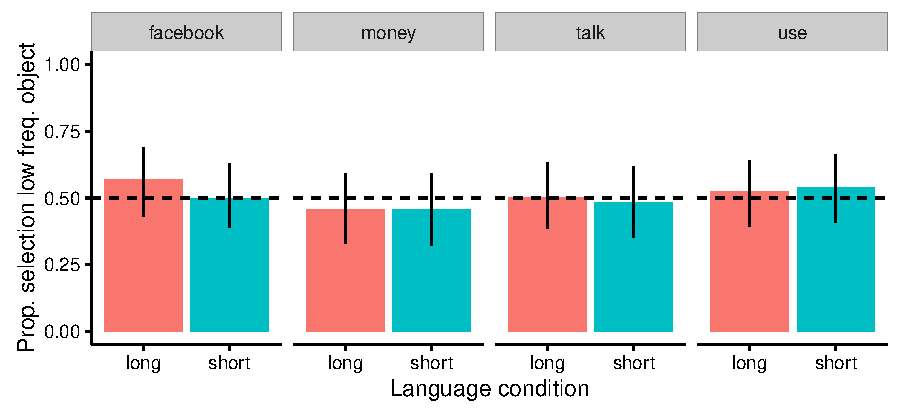
\includegraphics[width=6in]{figs/fact_plots.pdf}
  \caption{\label{fig:fact_plots} Experiment 6 results: Proportion participants selecting the object associated with the low frequency fact as a function of fact category and language condition. See Table \ref{tab:facts} for explanation of fact categories. Error bars are bootstrapped 95\% confidence intervals.}
 \end{center}
\end{figure}

\section{Experiment 7: Exemplar variability}
The final hypothesis about conceptual complexity derives from the Prototype Theory of concepts: A concept is conceptually complex if its exemplars are highly variable. This is predicted by 

cite haskell

\subsection{Methods}
\subsubsection{Participants}

396 participants completed the experiment.

\subsubsection{Stimuli} 
The linguistic stimuli were identical to previous experiments. There were four classes of object stimuli (bugs, birds, flowers, and fish). Each participant saw 10 objects from two classes. For each object class, two features varied continuously (e.g. for bugs, body and head size). Size parameters for the low variability objects were  sampled from a low variability distribution, and size parameters for the high variability objects were  sampled from a high variability distribution (see Fig.\ \ref{fig:var_screen_shot} for sample stimuli sets).

\subsubsection{Procedure}
The procedure was identical to Exp. 5a, with the exception of the training display. During the training phase, participants were given the following instructions:

\begin{quote}
In the country of Desodonia, there are two different \{forests/forests/fields/lakes\}. Each \{forest/forest/field/lake\}  is home to a different kind of \{bug/bird/flower/fish\}. To see some of the \{bugs/birds/flowers/fish\} in each \{forest/forest/field/lake\}, click the question marks below.
\end{quote}

They then saw two 5-by-2 grids of question marks corresponding to two different forests, fields, or lakes. The object was revealed after the participant clicked on the question mark. After all question marks had been clicked, the final display appeared as in Fig.\ \ref{fig:var_screen_shot}. After this training phase, participants advanced to a single word mapping trial as in Exp. 5a. 


  \begin{figure}
 \begin{center}
  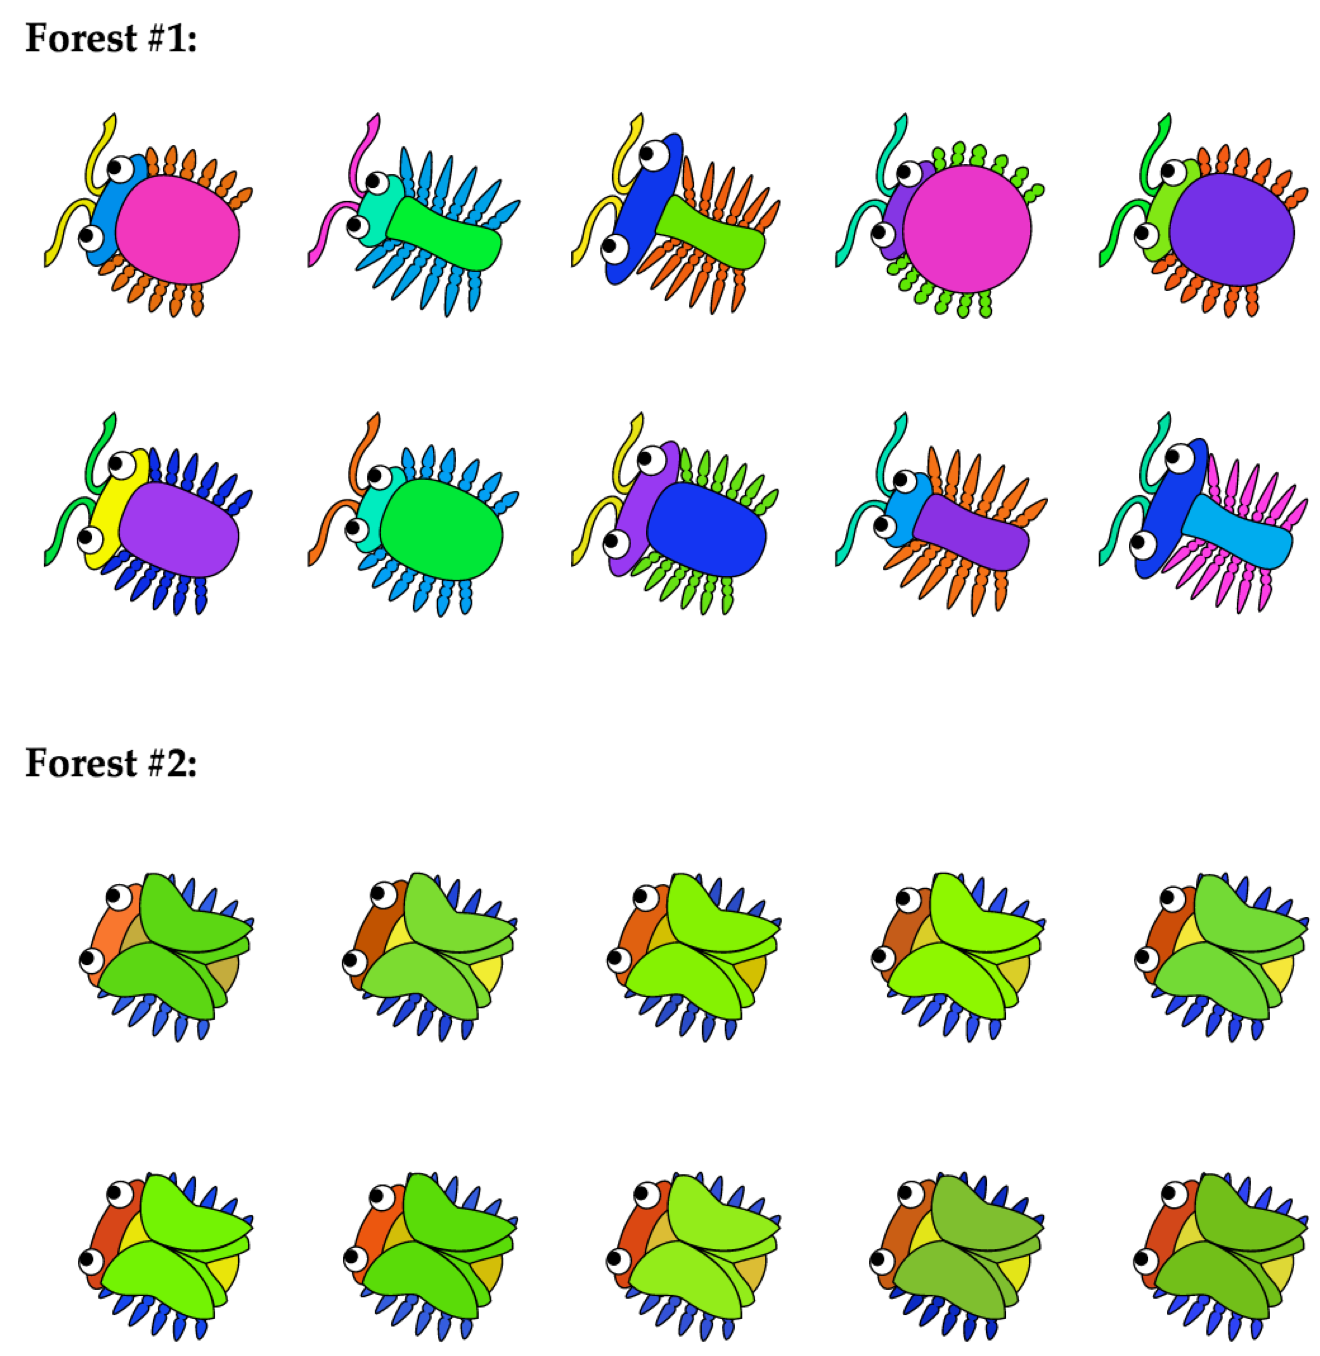
\includegraphics[width=4in]{figs/var_screen_shot.png}
  \caption{\label{fig:var_screen_shot} Example stimuli sets in Experiment 7. High variability bugs are shown on top (Forest \#1) and low variability on bottom (Forest \# 2).}
 \end{center}
\end{figure}



\subsection{Results and Discussion}

Selections of the high variability object did not differ as a function of word length (${\chi}^2$$(1) = 1.12$, $p = .29$; Fig.\ \ref{fig:var_plot}). However, 70 participants failed to correctly recall which category member was from the high-variability category, suggesting that participants may not have even noticed the critical manipulation. Nevertheless, even with these participants excluded, there was no difference between conditions (${\chi}^2$$(1) = .05$, $p = .82$).

  \begin{figure}
 \begin{center}
  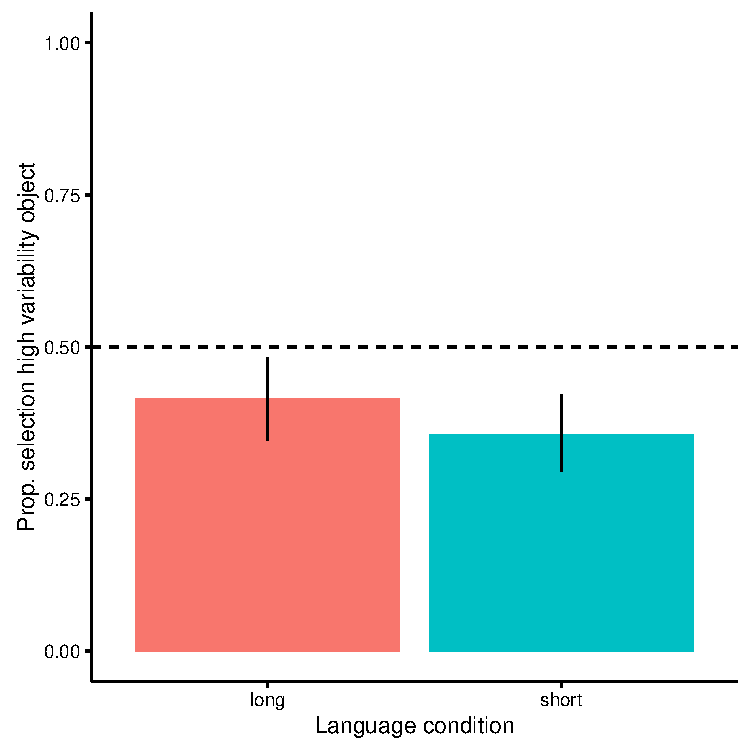
\includegraphics[width=4in]{figs/var_results.pdf}
  \caption{\label{fig:var_plot} Experiment 7 results: Proportion participants selecting the object associated with the high variability fact as a function language condition.  Error bars are bootstrapped 95\% confidence intervals.}
 \end{center}
\end{figure}

\subsection{Conclusion}









